\subsubsection{Poziom 1}

\clearpage
\begin{figure}[H]
	\centering
	\includepdf[pages={1}, angle=90]{img/DFD/1_level-eps-converted-to.pdf}
\end{figure}
\clearpage

\linespread{1.6}

%DFD1
\textbf{Opis}\\
Digram pokazuje wyodrębnienie podsystemów, które są przedstawione bardziej szczegółowo na kolejnych diagramach.


%DFD3 - Obsługa magazynu
\begin{figure}[H]
	\centering
	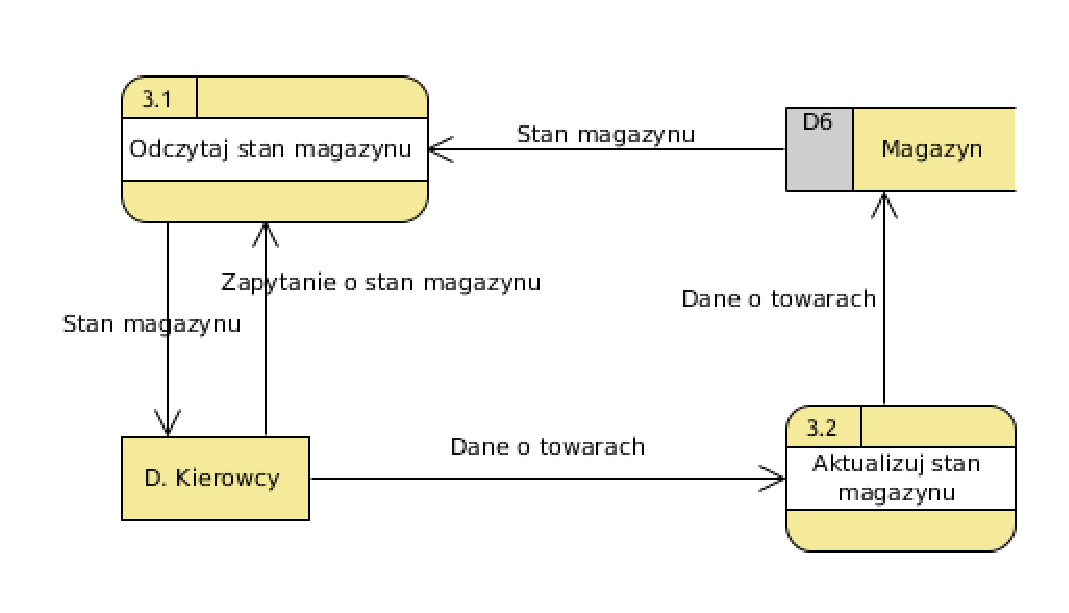
\includegraphics[width=\textwidth]{img/DFD3.eps}
\end{figure}

\textbf{Opis} \\
\underline{3.1 Odczytaj stan magazynu}\\
Kierowca odczytuje stan magazynu.
\textbf{Strumień wejściowy} zapytanie o stan magazynu\\
\textbf{Strumień wyjściowy} aktualny stan magazynu\\
\underline{3.2 Aktualizuj stan magazynu}\\ 
Stan magazynu jest aktualizowany na podstawie ilości produktów dostarczanych lub odbieranych.\\	
\textbf{Strumień wejściowy} Produkty przyjmawane do magazynu, produkty wydawane przez magazyn.